\chapter{TPC \textit{Benchmark} H}
\label{tpch}

A essência de um \textit{benchmark} é identificar e definir os melhores padrões de excelência para produtos, serviços e/ou processos, e então realizar aperfeiçoamentos de forma que esses padrões sejam alcançados \cite{bhutta1999benchmarking}. De maneira geral, \textit{benchmarks} se consolidaram como uma ferramenta para melhorar o desempenho de organizações e a competitividade nos negócios \cite{kyro2003revising}.

O TPC \textit{\textit{benchmark}} H é um padrão de decisão de negócio internacionalmente aceito para comparações de desempenho entre SGBDs utilizados em ambientes OLAP criado pela organização TPC. De acordo com a página oficial do TPC\footnote{http://www.tpc.org/information/about/abouttpc.asp}, esta organização sem fins lucrativos foi fundada com o objetivo de definir padrões para \textit{benchmarks} no processamento de transações e bancos de dados. Ela é responsável pelo desenvolvimento e atualização destes \textit{benchmarks}, bem como pela divulgação dos resultados apresentados por eles. Entre os sócios\footnote{Lista de sócios acessada em Junho de 2017} responsáveis por isto estão as empresas Dell, Hewlet Packard, IBM, Microsoft, Oracle, Intel e Cisco. A lista de todos os sócios pode ser acessada na página oficial da organização.

Alguns trabalhos já foram realizados utilizando o TPC-H \cite{ngamsuriyaroj2010performance, nadee2012performance, thanopoulou2012benchmarking, barata2014ycsb, rutishauser2012tpc, soares2012avaliaccao}. Ngamsuriyaroj e Pornpattana \cite{ngamsuriyaroj2010performance} aplicam as consultas do TPC-H no MySQL Cluster a fim de avaliar seu desempenho. O trabalho de Nadee e Ngamsuriyaroj \cite{nadee2012performance} tem uma proposta parecida com o primeiro \cite{ngamsuriyaroj2010performance}, porém o intuito é avaliar o desempenho de um \textit{cluster} Java EE baseado nas características das consultas do TPC-H. Thanopoulou et al. \cite{thanopoulou2012benchmarking} foca em aplicar o TPC-H em bancos de dados de pequenas empresas que não podem arcar com configurações de \textit{hardware} melhores para administrar um banco de dados. Barata, Bernardino e Furtado \cite{barata2014ycsb} fazem uma descrição teórica de dois \textit{benchmarks}, o YCSB (\textit{Yahoo Cloud Serving Benchmark}), voltado para a área de \textit{Big Data}, e o TPC-H. Rutishauser e Noureldin \cite{rutishauser2012tpc} realizam uma análise comparativa entre PostgreSQL e MongoDB aplicando o TPC-H. O primeiro é um SGBD relacional clássico, e o outro um SGBD NoSQL com algumas consultas do TPC-H adaptadas. Por fim, Soares \cite{soares2012avaliaccao} compara SGBD relacionais e colunares executando um teste de força sob o \textit{Star Schema Benchmark} simulando bases de dados de 1Gb, 2Gb, 5Gb e 10Gb.

De acordo com o manual de especificação fornecido pelo TPC \cite{tpc2017specs}, o TPC-H é um \textit{\textit{benchmark}} de suporte à decisão de negócios, constituído de uma série de consultas comerciais \textit{ad-hoc} e modificações simultâneas de dados com finalidade de retratar a realidade das empresas. Ele representa DSS que examinam grandes volumes de dados; executam consultas com um alto grau de complexidade; e respondem questões críticas de negócio. Como o \textit{\textit{benchmark}} trata de grandes volumes de dados, o tamanho mínimo de banco de dados proposto pelo TPC-H é de 1GB, seguido por 10GB, 30GB, 100GB, 300GB, 1000GB, 3000GB, 10000GB, 30000GB e 100000GB. Estes valores também correspondem ao Fator de Escala (\textit{Factor Scale} -- SF). 

Com o intuito de avaliar o resultado do desempenho de SGBDs como DW, é necessário ter conhecimento de como os dados que irão popular o DW estão distribuídos. Para tal, o TPC-H propõe um ambiente normalizado \textit{Snow Flake}. Ele é composto por oito tabelas e é descrito na Seção \ref{ambiente_1}. Do mesmo modo, a fim de obedecer as regras de modelagem deste ambiente, é preciso ter dados conhecidos para popular os DWs. Estes dados são fornecidos pelo \textit{software} DBGen.

O DBGen foi implementado pelo TPC-H, com o objetivo de realizar a população de dados em um DW seguindo a modelagem original \textit{Snow Flake}. São gerados oito arquivos separados no formato \texttt{<nome da tabela>.tbl} -- exemplificando, a tabela de dados \textit{Part} será gerada como \texttt{part.tbl}; onde as linhas de cada arquivo representam as tuplas dentro da respectiva tabela, tendo seus atributos separados por um delimitador \textit{pipe} ("$\mid$"). Por padrão, os arquivos são gerados para uma base de dados da classe de 1GB, quando nenhum SF é especificado.

Assim como é necessário conhecer os dados de modo a seguir a modelagem proposta pelo \textit{benchmark}, é preciso formular consultas que visam responder às questões de negócio definidas pelo TPC-H sobre o modelo de dados. O próprio TPC define para seu modelo 22 consultas, cada qual definida por (i) uma questão de negócio, que ilustra o contexto no qual a consulta pode ser aplicada; (ii) uma definição funcional, que corresponde à implementação da consulta utilizando a Linguagem SQL-92; (iii) parâmetros de substituição, que geram os valores necessários para completar os parâmetros da consulta; e (iv) validação, que descreve como validar a consulta no BD. Igualmente à geração de dados, a geração de consultas também é feita com o uso de um programa fornecido pelo TPC, o QGen.

Com o QGen é possível gerar as consultas de acordo com a especificação do TPC-H inserindo os parâmetros de substituição adequados em cada uma. A Consulta 1 presente no Apêndice \ref{queries_1}, Consulta de Relatório de Resumo de Preços, possui o parâmetro de substituição [DELTA], correspondente a um número inteiro entre 60 e 120, inserido ao executar o programa QGen para a respectiva consulta. Esses valores podem ser inseridos de maneira aleatória, entretanto o TPC-H define valores padrão para os parâmetros de substituição para fins de validação; portanto as consultas no QGen são geradas utilizando os valores padrão. As 22 consultas com suas respectivas questões de negócio e parâmetros de substituição são descritas no Apêndice \ref{queries_1}.

\section{Metodologia}
\label{metodologia}

Após a geração dos arquivos é criado em cada SGBD um esquema correspondente às classes utilizadas, tanto para o Ambiente Normalizado quanto para o Desnormalizado. Cada SGBD é então executado sobre os dois ambientes propostos. Em cada ambiente será executado o teste de performance, que consiste de duas execuções: o Teste de Força (\textit{Power Test}) e o Teste de Vazão (\textit{Throughput Test}), descritos nas Subseções \ref{power_test} e \ref{through_test}, respectivamente. O tempo resultante de cada etapa é utilizado para calcular o desempenho final do SGBD, medido em \textit{QphH@Size} -- quantidade de consultas executadas por hora, dada uma classe de tamanho de banco de dados. Uma execução é composta por:

\begin{itemize}
	\item \textit{SF}, que representa a classe do banco de dados.
	\item \textit{$Q_{i}$}, que representa uma consulta, onde \mbox{$1 \le i \le 22$}.
	\item \textit{S}, que define o número de sessões de consulta do Teste de Vazão.
	\item \textit{s}, que representa uma dada sessão, onde \mbox{$1 \le s \le S$}.
	\item \textit{$T_{s}$}, que representa o tempo, em segundos, resultante do processo inteiro.
	\item \textit{$RF_{j}$}, que representa a Função de Atualização (\textit{Refresh Function} -- RF), onde:
		\begin{itemize}
		    \item RF1: inserção de novos registros. O número de registros inseridos deve ser igual para o número de registros removidos pela RF2. O pseudocódigo para a RF1 é como:
		
\begin{verbatim}
    loop (SF * 1500) times
        insert <new row into> ORDERS table
        loop random(1, 7) times
            insert <new row into> LINEITEM table
        end loop
    end loop
\end{verbatim}
		    \item RF2: remoção de registros antigos. O pseudocódigo para a RF1 é como:
		
\begin{verbatim}
    loop (SF * 1500) times
        delete from ORDERS where O_ORDERKEY = [valor]
        delete from LINEITEM where I_ORDERKEY = [valor]
    end loop
\end{verbatim}
		\end{itemize}
\end{itemize}

O conjunto de dados para executar com sucesso as RFs também são gerados pelo DBGen utilizando a \textit{flag} -U.

\subsection{Teste de Força}
\label{power_test}
O Teste de Força objetiva medir a execução de uma dada consulta do sistema com um único usuário ativo. Neste teste é criada uma única sessão com o respectivo SGBD e as seguintes instruções são executadas:

\begin{itemize}
	\item Execução da RF1.
	\item Execução de cada consulta proposta pelo TPC-H, ou adaptada, de forma sequencial uma única vez até a última consulta.
	\item Execução da RF2.
\end{itemize}

Será armazenado ao fim do teste o tempo em segundos resultante de cada consulta, bem como o tempo de execução de cada função. Este resultado será utilizado na Equação \ref{eq:1}.

\begin{myequation}%
\label{eq:1}
{\scriptstyle Power@Size} = \frac{3600 * SF}{\sqrt[24]{\prod_{i = 2}^{i = 22}Q(i, 0) * \prod_{j = 1}^{j = 2}RF(j, 0)}} %
\end{myequation}
%

\subsection{Teste de Vazão}
\label{through_test}
Este teste mede a capacidade do sistema de processar a maior quantidade possível de consultas no menor intervalo de tempo. Aqui o TPC-H exige um número mínimo de sessões de consulta de acordo com a classe de tamanho do banco de dados, como mostra a Tabela \ref{min_sessions}.

\begin{table}[htpb]
\centering
\caption{Número mínimo de sessões para uma classe de banco de dados}
\label{min_sessions}
\begin{tabular}{|c|c|}
\hline
\multicolumn{1}{|c|}{\textbf{Classe do Banco de Dados}} & \textbf{Número de Sessões} \\ \hline
1 GB                                      & 2                            \\ \hline
10 GB                                      & 3                          \\ \hline
30 GB                                        & 4                             \\ \hline
100 GB                                        & 5                             \\ \hline
300 GB                                        & 6                             \\ \hline
1000 GB                                        & 7                             \\ \hline
3000 GB                                        & 8                             \\ \hline
10000 GB                                        & 9                             \\ \hline
30000 GB                                        & 10                             \\ \hline
100000 GB                                        & 11                             \\ \hline
\end{tabular}
\end{table}

É criada uma sessão para executar as Funções e \textit{N} sessões para executar as consultas, de acordo com a Tabela \ref{min_sessions}. As instruções são executadas concorrentemente. Para a sessão das Funções, as seguintes instruções são executadas:

\begin{itemize}
	\item A RF1 e RF2 deverão ser executadas sequencialmente \textit{N} vezes, onde \textit{N} é o número de sessões para a execução de consultas.
	\item Para cada sessão de consultas, cada consulta será executada sequencialmente até a última.
\end{itemize}

Ao fim do teste, é armazenado o tempo em segundos da execução do processo inteiro. O processo inicia quando a primeira sessão, seja de consulta ou de Função, executa sua instrução e finaliza quando a última sessão recebe uma resposta. O resultado é utilizado para calcular o desempenho do SGBD para o Teste de Vazão conforme a Equação \ref{eq:2}.

\begin{myequation}%
\label{eq:2}
{\scriptstyle Throughput@Size} = \frac{S * 22 * 3600}{T_s * SF} %
\end{myequation}
%

O resultado dos cálculos de Força e Vazão serão utilizados para calcular o desempenho final do SGBD da seguinte forma:

\begin{myequation}%
\label{eq:3}
{ \scriptstyle QphH@Size = \sqrt{Power@Size * Throughput@Size} } %
\end{myequation}
%

\section{Ambiente Original Normalizado}
\label{ambiente_1}

O modelo de ambiente proposto pelo TPC-H é um esquema normalizado \textit{Snow Flake}. Ele é composto por oito tabelas, sendo que destas, seis têm o tamanho multiplicado por um Fator de Escala, que corresponde ao tamanho da classe do banco de dados; enquanto que as demais, \textit{NATION} e \textit{REGION}, têm tamanho fixo. O relacionamento \textit{one-to-many} entre as tabelas do esquema \textit{Snow Flake} é apresentado na Figura \ref{fig:snow_flake}, adaptada do manual de especificação do TPC-H \cite{tpc2017specs}.

\begin{figure*}[h]
	\centering
		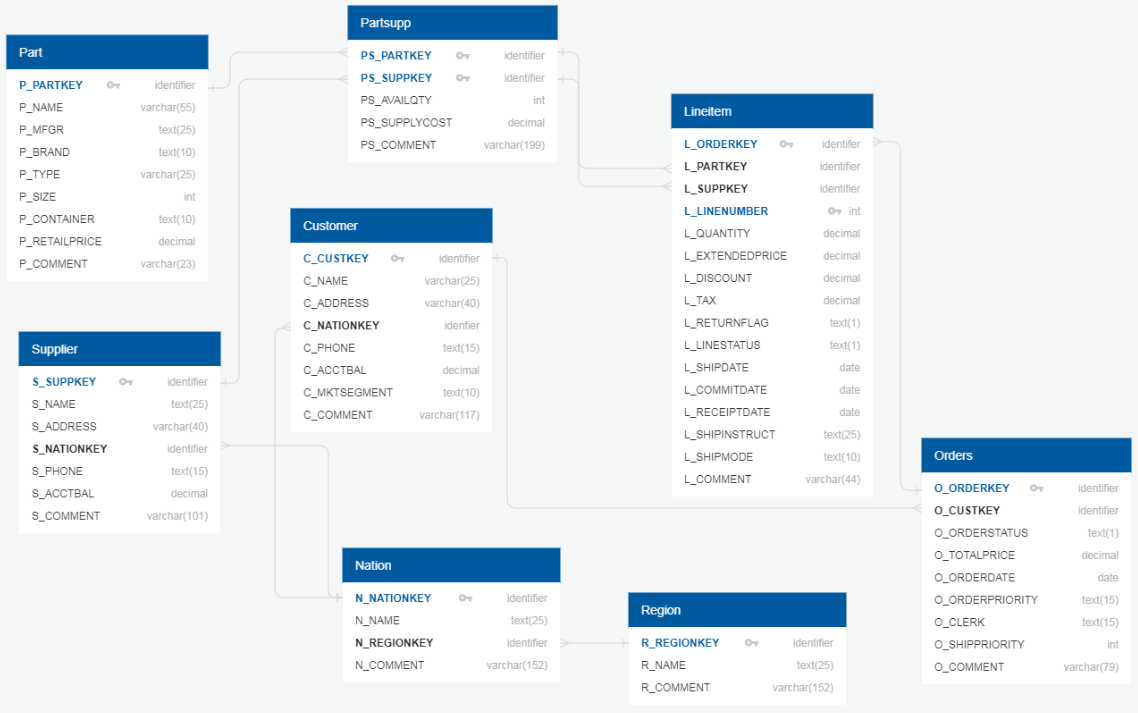
\includegraphics[width=\textwidth]{img/snow_flake.png}
	\caption{Esquema do ambiente normalizado}
	\label{fig:snow_flake}
\end{figure*}

\begin{comment}
\begin{table}[h]
\centering
\caption{Dados para a classe de 1GB}
\label{1gb_table}
\begin{tabular}{|l|c|c|}
\hline
\multicolumn{1}{|c|}{\textbf{Nome da tabela}} & \textbf{Cardinalidade} & \textbf{Tamanho} \\ \hline
CUSTOMER                                      & 150 K                  & 23.3 MB          \\ \hline
LINEITEM                                      & 6 M                    & 730 MB           \\ \hline
NATION                                        & 25                     & 2.19 KB          \\ \hline
ORDERS                                        & 1.5 M                  & 165 MB           \\ \hline
PART                                          & 200 K                  & 23.2 MB          \\ \hline
PARTSUPP                                      & 800 K                  & 114 MB           \\ \hline
REGION                                        & 5                      & 394 Bytes        \\ \hline
SUPPLIER                                      & 10 K                   & 1.35 MB          \\ \hline
Total																					&												 & 								\\ \hline
\end{tabular}
\end{table}

\begin{table}[h]
\centering
\caption{Dados para a classe de 10GB}
\label{10gb_table}
\begin{tabular}{|l|c|c|}
\hline
\multicolumn{1}{|c|}{\textbf{Nome da tabela}} & \textbf{Cardinalidade} & \textbf{Tamanho} \\ \hline
CUSTOMER                                      & 1.5 M                  & 234 MB          	\\ \hline
LINEITEM                                      & 60 M                   & 7.29 GB          \\ \hline
NATION                                        & 25                     & 2.19 KB          \\ \hline
ORDERS                                        & 15 M                   & 1.64 GB          \\ \hline
PART                                          & 2 M                  	 & 233 MB          	\\ \hline
PARTSUPP                                      & 8 M                  	 & 1.12 GB          \\ \hline
REGION                                        & 5                      & 394 Bytes        \\ \hline
SUPPLIER                                      & 100 K                  & 13.6 MB          \\ \hline
Total																					&												 & 								\\ \hline
\end{tabular}
\end{table}

\begin{table}[h]
\centering
\caption{Dados para a classe de 30GB}
\label{30gb_table}
\begin{tabular}{|l|c|c|}
\hline
\multicolumn{1}{|c|}{\textbf{Nome da tabela}} & \textbf{Cardinalidade} & \textbf{Tamanho} \\ \hline
CUSTOMER                                      & 4.5 m                  & 706 MB           \\ \hline
LINEITEM                                      & 180 M                  & 22.1 GB          \\ \hline
NATION                                        & 25                     & 2.19 KB          \\ \hline
ORDERS                                        & 450 M                  & 4.97 GB          \\ \hline
PART                                          & 6 M                  	 & 704 MB           \\ \hline
PARTSUPP                                      & 24 M                   & 3.41 GB          \\ \hline
REGION                                        & 5                      & 394 Bytes        \\ \hline
SUPPLIER                                      & 30 K                   & 41 MB            \\ \hline
Total																					&												 & 								\\ \hline
\end{tabular}
\end{table}
\end{comment}

Os tipos de dados atribuídos aos atributos de uma entidade podem ser:

\begin{itemize}
    \item Identificador: \textit{identifier} -- corresponde a um inteiro que define a PK de uma entidade
    \item Inteiro: int
    \item Decimal: decimal
    \item Texto fixo de tamanho N: text(N)
    \item Texto variável de tamanho N: varchar(N)
    \item Data: date
    
\end{itemize}

Detalhes sobre as consultas implementadas na Linguagem SQL relacionadas a esse ambiente são encontradas no Apêndice \ref{queries_1}.

\section{Ambiente Desnormalizado}

Embora modelos de dados normalizados sejam eficientes em processos operacionais, SGBDs relacionais não executam uma consulta de maneira eficiente em um esquema normalizado \cite{kimball2002dw}. A otimização é afetada pelo número de \textit{joins}, o que vai contra um dos objetivos de um \textit{warehouse}: recuperação de dados com rapidez. 

As modificações no modelo do Ambiente Normalizado se fundamentaram na criação de um modelo parecido com o apresentado pela modelagem \textit{Star}, com uma Tabela Fato central descrita por Tabelas Dimensão. Também procurou-se eliminar quaisquer tabelas cujos atributos sejam frequentemente utilizados em operações de \textit{join}, alguns característicos de um modelo com Tabelas Subdimensionais, e que possam ser incluídos nas tabelas que possuam relacionamento com eles. O esquema final do modelo \textit{Star} é mostrado na Figura \ref{fig:star}.

\begin{figure*}[h]
	\centering
		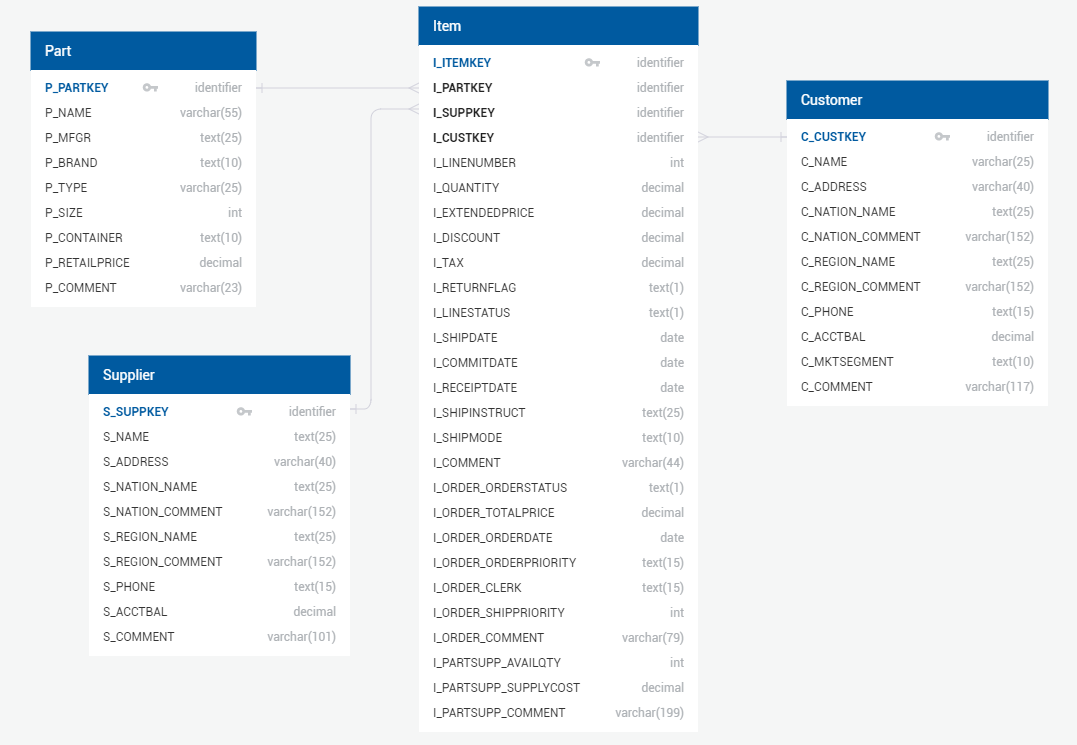
\includegraphics[width=\textwidth]{img/star.png}
	\caption{Esquema do ambiente desnormalizado}
	\label{fig:star}
\end{figure*}
 
A primeira modificação no modelo \textit{Snow Flake} foi a exclusão das entidades Dimensão \textit{Nation} e \textit{Region}. Essas entidades são Tabelas Subdimensionais das entidades \textit{Customer} e \textit{Supplier}, sendo frequentemente requeridas quando há a necessidade de consultar a nação e/ou a região de um cliente e/ou de um fornecedor, assim optou-se por incluir os atributos \texttt{N\_NAME, N\_COMMENT, R\_NAME} e \texttt{R\_COMMENT} nas entidades \textit{Supplier} e \textit{Customer}. 

Com a intenção de criar uma única Tabela Fato no esquema desnormalizado, observou-se (i) a possibilidade de unir as entidades \textit{Lineitem} e \textit{Orders} em uma única entidade nomeada como \textit{Item}, visto que as duas possuem um relacionamento. Isto também eliminaria alguns \textit{joins} realizados entre as duas entidades nas consultas listadas no Apêndice \ref{queries_1}. A PK \texttt{C\_CUSTKEY} de \textit{Customer} que antes estava em \textit{Orders} como FK é transferida agora para \textit{Item}. Também nota-se que (ii) as entidades \textit{Part} e \textit{Supplier} têm suas PKs como FKs na entidade antes denominada \textit{Lineitem}, provenientes da entidade intermediária \textit{Partsupp}. Optou-se assim por incluir os atributos de \textit{Partsupp} na nova entidade \textit{Item}, excluindo a primeira do esquema e mantendo o relacionamento de \textit{Supplier} e \textit{Part} diretamente com \textit{Item}, através das chaves \texttt{P\_PARTKEY} e \texttt{S\_SUPPKEY}.

O esquema final agora possui uma Tabela Fato, \textit{Item}; e três tabelas Dimensão, \textit{Part}, \textit{Customer} e \textit{Supplier}, cada qual com sua chave mantendo o relacionamento com a tabela \textit{Item}. Os dados presentes nas entidades são do mesmo tipo descritos na Seção \ref{ambiente_1}. As consultas em Linguagem SQL relacionadas a esse ambiente são encontradas no Apêndice \ref{queries_2}.

A inserção dos dados do Ambiente Desnormalizado será realizada após todos os dados gerados pelo DBGen do Ambiente Normalizado terem sido populados nos SGBDs. Com isso, é possível realizar \textit{joins} de acordo com as mudanças e o resultado destes será armazenado no esquema correspondente. Por exemplo, ao realizar um \textit{join} entre as entidades \textit{Nation} e \textit{Region} selecionando todos os seus atributos, estes são enviados como entrada para a inserção em uma nova tabela do esquema Desnormalizado correspondente, digamos, \textit{Nation\_Region}. Após, é realizado um novo \textit{join} com as entidades \textit{Supplier} e \textit{Part}, separadamente, para incluir os atributos de \textit{Nation\_Region}: \texttt{N\_NAME, N\_COMMENT, R\_NAME} e \texttt{R\_COMMENT}; bem como os atributos originais das duas entidades anteriores, nas novas entidades \textit{Supplier} e \textit{Part}.